% Created by tikzDevice version 0.10.1 on 2018-02-07 11:01:35
% !TEX encoding = UTF-8 Unicode
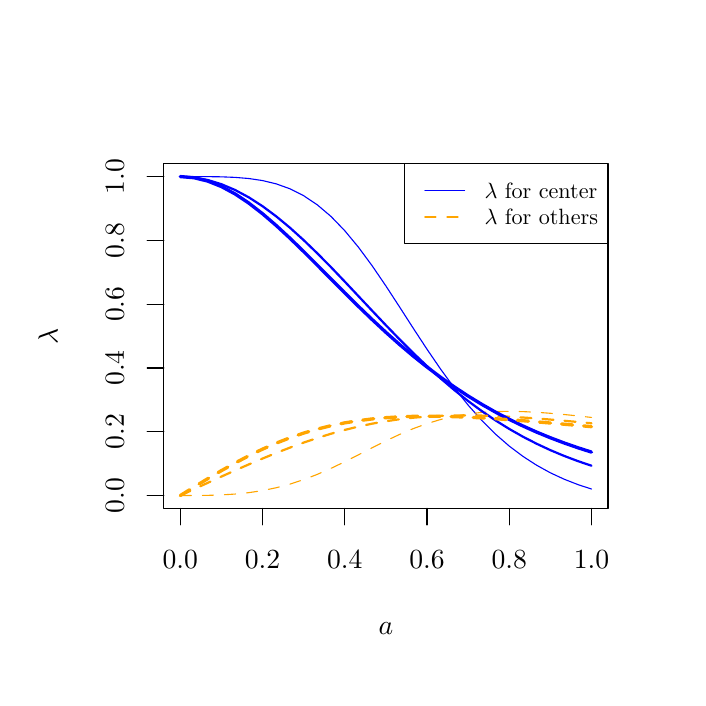
\begin{tikzpicture}[x=1pt,y=1pt]
\definecolor{fillColor}{RGB}{255,255,255}
\path[use as bounding box,fill=fillColor,fill opacity=0.00] (0,0) rectangle (234.88,234.88);
\begin{scope}
\path[clip] ( 49.20, 61.20) rectangle (209.68,185.68);
\definecolor{drawColor}{RGB}{0,0,255}

\path[draw=drawColor,line width= 0.4pt,line join=round,line cap=round] ( 55.14,181.07) --
	( 60.10,181.07) --
	( 65.05,181.05) --
	( 70.00,180.98) --
	( 74.96,180.78) --
	( 79.91,180.37) --
	( 84.86,179.63) --
	( 89.81,178.44) --
	( 94.77,176.66) --
	( 99.72,174.17) --
	(104.67,170.85) --
	(109.63,166.64) --
	(114.58,161.51) --
	(119.53,155.54) --
	(124.49,148.82) --
	(129.44,141.55) --
	(134.39,133.95) --
	(139.34,126.25) --
	(144.30,118.68) --
	(149.25,111.44) --
	(154.20,104.67) --
	(159.16, 98.48) --
	(164.11, 92.92) --
	(169.06, 87.99) --
	(174.02, 83.68) --
	(178.97, 79.96) --
	(183.92, 76.76) --
	(188.87, 74.03) --
	(193.83, 71.73) --
	(198.78, 69.79) --
	(203.73, 68.16);
\end{scope}
\begin{scope}
\path[clip] (  0.00,  0.00) rectangle (234.88,234.88);
\definecolor{drawColor}{RGB}{0,0,0}

\path[draw=drawColor,line width= 0.4pt,line join=round,line cap=round] ( 55.14, 61.20) -- (203.73, 61.20);

\path[draw=drawColor,line width= 0.4pt,line join=round,line cap=round] ( 55.14, 61.20) -- ( 55.14, 55.20);

\path[draw=drawColor,line width= 0.4pt,line join=round,line cap=round] ( 84.86, 61.20) -- ( 84.86, 55.20);

\path[draw=drawColor,line width= 0.4pt,line join=round,line cap=round] (114.58, 61.20) -- (114.58, 55.20);

\path[draw=drawColor,line width= 0.4pt,line join=round,line cap=round] (144.30, 61.20) -- (144.30, 55.20);

\path[draw=drawColor,line width= 0.4pt,line join=round,line cap=round] (174.02, 61.20) -- (174.02, 55.20);

\path[draw=drawColor,line width= 0.4pt,line join=round,line cap=round] (203.73, 61.20) -- (203.73, 55.20);

\node[text=drawColor,anchor=base,inner sep=0pt, outer sep=0pt, scale=  1.00] at ( 55.14, 39.60) {0.0};

\node[text=drawColor,anchor=base,inner sep=0pt, outer sep=0pt, scale=  1.00] at ( 84.86, 39.60) {0.2};

\node[text=drawColor,anchor=base,inner sep=0pt, outer sep=0pt, scale=  1.00] at (114.58, 39.60) {0.4};

\node[text=drawColor,anchor=base,inner sep=0pt, outer sep=0pt, scale=  1.00] at (144.30, 39.60) {0.6};

\node[text=drawColor,anchor=base,inner sep=0pt, outer sep=0pt, scale=  1.00] at (174.02, 39.60) {0.8};

\node[text=drawColor,anchor=base,inner sep=0pt, outer sep=0pt, scale=  1.00] at (203.73, 39.60) {1.0};

\path[draw=drawColor,line width= 0.4pt,line join=round,line cap=round] ( 49.20, 65.81) -- ( 49.20,181.07);

\path[draw=drawColor,line width= 0.4pt,line join=round,line cap=round] ( 49.20, 65.81) -- ( 43.20, 65.81);

\path[draw=drawColor,line width= 0.4pt,line join=round,line cap=round] ( 49.20, 88.86) -- ( 43.20, 88.86);

\path[draw=drawColor,line width= 0.4pt,line join=round,line cap=round] ( 49.20,111.91) -- ( 43.20,111.91);

\path[draw=drawColor,line width= 0.4pt,line join=round,line cap=round] ( 49.20,134.96) -- ( 43.20,134.96);

\path[draw=drawColor,line width= 0.4pt,line join=round,line cap=round] ( 49.20,158.02) -- ( 43.20,158.02);

\path[draw=drawColor,line width= 0.4pt,line join=round,line cap=round] ( 49.20,181.07) -- ( 43.20,181.07);

\node[text=drawColor,rotate= 90.00,anchor=base,inner sep=0pt, outer sep=0pt, scale=  1.00] at ( 34.80, 65.81) {0.0};

\node[text=drawColor,rotate= 90.00,anchor=base,inner sep=0pt, outer sep=0pt, scale=  1.00] at ( 34.80, 88.86) {0.2};

\node[text=drawColor,rotate= 90.00,anchor=base,inner sep=0pt, outer sep=0pt, scale=  1.00] at ( 34.80,111.91) {0.4};

\node[text=drawColor,rotate= 90.00,anchor=base,inner sep=0pt, outer sep=0pt, scale=  1.00] at ( 34.80,134.96) {0.6};

\node[text=drawColor,rotate= 90.00,anchor=base,inner sep=0pt, outer sep=0pt, scale=  1.00] at ( 34.80,158.02) {0.8};

\node[text=drawColor,rotate= 90.00,anchor=base,inner sep=0pt, outer sep=0pt, scale=  1.00] at ( 34.80,181.07) {1.0};

\path[draw=drawColor,line width= 0.4pt,line join=round,line cap=round] ( 49.20, 61.20) --
	(209.68, 61.20) --
	(209.68,185.68) --
	( 49.20,185.68) --
	( 49.20, 61.20);
\end{scope}
\begin{scope}
\path[clip] (  0.00,  0.00) rectangle (234.88,234.88);
\definecolor{drawColor}{RGB}{0,0,0}

\node[text=drawColor,anchor=base,inner sep=0pt, outer sep=0pt, scale=  1.00] at (129.44, 15.60) {$a$};

\node[text=drawColor,rotate= 90.00,anchor=base,inner sep=0pt, outer sep=0pt, scale=  1.00] at ( 10.80,123.44) {$\lambda$};
\end{scope}
\begin{scope}
\path[clip] ( 49.20, 61.20) rectangle (209.68,185.68);
\definecolor{drawColor}{RGB}{255,165,0}

\path[draw=drawColor,line width= 0.4pt,dash pattern=on 4pt off 4pt ,line join=round,line cap=round] ( 55.14, 65.81) --
	( 60.10, 65.82) --
	( 65.05, 65.88) --
	( 70.00, 66.04) --
	( 74.96, 66.35) --
	( 79.91, 66.86) --
	( 84.86, 67.61) --
	( 89.81, 68.63) --
	( 94.77, 69.94) --
	( 99.72, 71.56) --
	(104.67, 73.47) --
	(109.63, 75.65) --
	(114.58, 78.03) --
	(119.53, 80.54) --
	(124.49, 83.08) --
	(129.44, 85.57) --
	(134.39, 87.90) --
	(139.34, 90.00) --
	(144.30, 91.81) --
	(149.25, 93.30) --
	(154.20, 94.46) --
	(159.16, 95.30) --
	(164.11, 95.86) --
	(169.06, 96.16) --
	(174.02, 96.24) --
	(178.97, 96.14) --
	(183.92, 95.90) --
	(188.87, 95.54) --
	(193.83, 95.10) --
	(198.78, 94.59) --
	(203.73, 94.04);
\definecolor{drawColor}{RGB}{0,0,255}

\path[draw=drawColor,line width= 0.8pt,line join=round,line cap=round] ( 55.14,181.07) --
	( 60.10,180.76) --
	( 65.05,179.84) --
	( 70.00,178.32) --
	( 74.96,176.22) --
	( 79.91,173.56) --
	( 84.86,170.37) --
	( 89.81,166.70) --
	( 94.77,162.59) --
	( 99.72,158.11) --
	(104.67,153.33) --
	(109.63,148.31) --
	(114.58,143.12) --
	(119.53,137.86) --
	(124.49,132.58) --
	(129.44,127.36) --
	(134.39,122.25) --
	(139.34,117.31) --
	(144.30,112.59) --
	(149.25,108.11) --
	(154.20,103.89) --
	(159.16, 99.96) --
	(164.11, 96.32) --
	(169.06, 92.96) --
	(174.02, 89.88) --
	(178.97, 87.07) --
	(183.92, 84.53) --
	(188.87, 82.22) --
	(193.83, 80.14) --
	(198.78, 78.27) --
	(203.73, 76.59);
\definecolor{drawColor}{RGB}{255,165,0}

\path[draw=drawColor,line width= 0.8pt,dash pattern=on 4pt off 4pt ,line join=round,line cap=round] ( 55.14, 65.81) --
	( 60.10, 68.11) --
	( 65.05, 70.40) --
	( 70.00, 72.67) --
	( 74.96, 74.90) --
	( 79.91, 77.07) --
	( 84.86, 79.18) --
	( 89.81, 81.21) --
	( 94.77, 83.13) --
	( 99.72, 84.94) --
	(104.67, 86.61) --
	(109.63, 88.15) --
	(114.58, 89.52) --
	(119.53, 90.74) --
	(124.49, 91.79) --
	(129.44, 92.67) --
	(134.39, 93.38) --
	(139.34, 93.94) --
	(144.30, 94.34) --
	(149.25, 94.61) --
	(154.20, 94.75) --
	(159.16, 94.78) --
	(164.11, 94.70) --
	(169.06, 94.54) --
	(174.02, 94.31) --
	(178.97, 94.01) --
	(183.92, 93.66) --
	(188.87, 93.27) --
	(193.83, 92.84) --
	(198.78, 92.40) --
	(203.73, 91.93);
\definecolor{drawColor}{RGB}{0,0,255}

\path[draw=drawColor,line width= 1.2pt,line join=round,line cap=round] ( 55.14,181.07) --
	( 60.10,180.66) --
	( 65.05,179.45) --
	( 70.00,177.47) --
	( 74.96,174.79) --
	( 79.91,171.48) --
	( 84.86,167.65) --
	( 89.81,163.39) --
	( 94.77,158.80) --
	( 99.72,153.99) --
	(104.67,149.04) --
	(109.63,144.04) --
	(114.58,139.05) --
	(119.53,134.16) --
	(124.49,129.39) --
	(129.44,124.79) --
	(134.39,120.39) --
	(139.34,116.20) --
	(144.30,112.25) --
	(149.25,108.52) --
	(154.20,105.04) --
	(159.16,101.78) --
	(164.11, 98.76) --
	(169.06, 95.95) --
	(174.02, 93.35) --
	(178.97, 90.95) --
	(183.92, 88.73) --
	(188.87, 86.70) --
	(193.83, 84.82) --
	(198.78, 83.10) --
	(203.73, 81.51);
\definecolor{drawColor}{RGB}{255,165,0}

\path[draw=drawColor,line width= 1.2pt,dash pattern=on 4pt off 4pt ,line join=round,line cap=round] ( 55.14, 65.81) --
	( 60.10, 68.88) --
	( 65.05, 71.89) --
	( 70.00, 74.81) --
	( 74.96, 77.58) --
	( 79.91, 80.18) --
	( 84.86, 82.58) --
	( 89.81, 84.75) --
	( 94.77, 86.68) --
	( 99.72, 88.38) --
	(104.67, 89.83) --
	(109.63, 91.06) --
	(114.58, 92.07) --
	(119.53, 92.87) --
	(124.49, 93.50) --
	(129.44, 93.95) --
	(134.39, 94.25) --
	(139.34, 94.43) --
	(144.30, 94.49) --
	(149.25, 94.45) --
	(154.20, 94.32) --
	(159.16, 94.13) --
	(164.11, 93.87) --
	(169.06, 93.57) --
	(174.02, 93.22) --
	(178.97, 92.85) --
	(183.92, 92.44) --
	(188.87, 92.02) --
	(193.83, 91.59) --
	(198.78, 91.15) --
	(203.73, 90.70);
\definecolor{drawColor}{RGB}{0,0,0}

\path[draw=drawColor,line width= 0.4pt,line join=round,line cap=round] (136.31,185.68) rectangle (209.68,156.88);
\definecolor{drawColor}{RGB}{0,0,255}

\path[draw=drawColor,line width= 0.4pt,line join=round,line cap=round] (143.51,176.08) -- (157.91,176.08);
\definecolor{drawColor}{RGB}{255,165,0}

\path[draw=drawColor,line width= 0.4pt,dash pattern=on 4pt off 4pt ,line join=round,line cap=round] (143.51,166.48) -- (157.91,166.48);
\definecolor{drawColor}{RGB}{0,0,0}

\node[text=drawColor,anchor=base west,inner sep=0pt, outer sep=0pt, scale=  0.80] at (165.11,173.32) {$\lambda$ for center};

\node[text=drawColor,anchor=base west,inner sep=0pt, outer sep=0pt, scale=  0.80] at (165.11,163.72) {$\lambda$ for others};
\end{scope}
\end{tikzpicture}
